\section{System and Problem Formulation}
\label{sec:system}

\begin{figure*}[t]
\centering
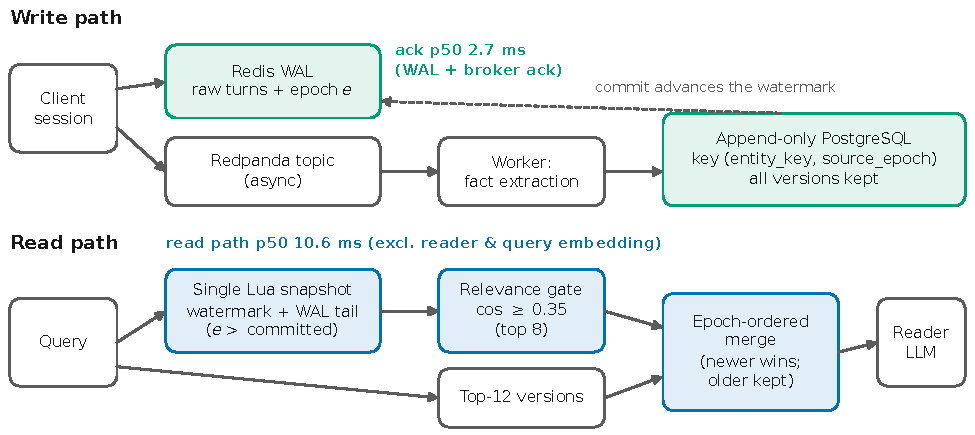
\includegraphics[width=\textwidth]{figures/fig1_architecture.pdf}
\caption{DeltaWAL-Versioned. \emph{Write path}: raw turns and a monotonic epoch $e$ are written through to a Redis WAL before the broker publish; the write is acknowledged after the WAL write and the broker acknowledgement (median \nm{fig1/write_ack_p50_ms}\,ms, Table~\ref{tab:latency}). A worker extracts facts into an append-only PostgreSQL/pgvector store keyed by (entity key, source epoch) and advances the committed watermark. \emph{Read path}: one Lua call snapshots the watermark and the uncommitted WAL tail; a cosine gate ($\tau=\nm{fig1/wal_sim_threshold}$, at most $m=\nm{frozen_config/wal_top_m}$ turns) selects relevant turns, which are merged with the top-$k$ stored versions ($k=\nm{frozen_config/top_k_facts}$) in epoch order under a newer-wins instruction, keeping older versions visible. Median read path \nm{fig1/read_path_p50_ms_excl_reader_and_query_embedding}\,ms, excluding the reader and the query embedding.}
\label{fig:arch}
\end{figure*}

\subsection{Setting}
\label{sec:setting}

\paragraph{Sessions, facts and the watermark.}
A user talks to an agent in sessions. When a session is written to memory it receives an epoch $e$ from a per-user counter that increases strictly in write order. A question $q$ arrives after the session with epoch $T$ has been written and acknowledged. An extractor $\phi$ maps each session to facts $f=(x, v, e)$: a normalised entity key $x$, a fact text $v$ and the source epoch $e$. In an asynchronous pipeline the write is acknowledged once the session is on a broker; a worker later runs $\phi$, embeds the facts and commits them to a vector store $M$. With $C$ the set of committed epochs, the committed watermark
\begin{equation}
W = \max\{\, w : e \in C \text{ for every epoch } e \le w \,\}
\end{equation}
is the largest epoch below which nothing is missing. At query time a system retrieves the top-$k$ stored items by cosine similarity to $q$, renders them into a prompt, and a reader LLM answers.

\paragraph{Lag and reordering.}
A deterministic barrier replaces wall-clock timing. At lag $\ell$, the in-flight set is $I_\ell = \{e : T-\ell < e \le T\}$ and every older session is committed; $\ell=0$ means the store is complete. To model stragglers, each older session is independently delayed, with probability $p_\text{ooo}$, to a uniformly random later commit slot. The in-flight tail does not depend on $p_\text{ooo}$, so the two fault axes are independent, and both are functions of the seed, the question and $(\ell, p_\text{ooo})$.

\paragraph{Store policies.}
When the worker commits $(x, v, e)$ and the store holds $(x, v', e')$, \emph{last-writer-wins} (LWW) replaces the old row unconditionally, \emph{compare-and-set} (CAS) replaces it only if $e > e'$ (a conditional upsert in PostgreSQL), and \emph{append} keeps both rows under the key $(x, e)$. LWW and CAS are in-place policies: after an update one value per key survives. They coincide when commits arrive in order. Under reordering, LWW can leave an older value in place. A key is \emph{updated} if at least two committed epochs wrote it and \emph{corrupted} if its stored epoch is below the newest committed epoch for that key; the out-of-order corruption rate (OOCR) is the corrupted fraction of updated keys.

\subsection{Two failure modes}
\label{sec:failures}

\paragraph{Read-after-write staleness.}
If the answer to $q$ depends on a fact from a session in $I_\ell$, typically an update, a system that reads only $M$ answers with the earlier value. This violates read-your-writes~\citep{terry1994session}: the write was acknowledged, yet the next read does not reflect it. A \emph{stale read} is a wrong answer to a knowledge-update question that matches the superseded value.

\paragraph{History erasure.}
Some questions ask about an earlier value, such as ``what was my previous goal''. Let key $x$ hold $v_\text{old}$ at epoch $e_\text{old}$ and $v_\text{new}$ at a later epoch. History is erased if $v_\text{old}$ cannot reach the reader. On the \emph{write side}, an in-place policy (LWW, CAS, or \memzero{}'s UPDATE) overwrites $v_\text{old}$ when $v_\text{new}$ commits, and no read path can recover it. On the \emph{read side}, a read path that masks stored items it believes superseded removes $v_\text{old}$ from the prompt although the store kept it. Both apply the rule ``keep only the newest value'', at different points.
A related failure is the \emph{missed merge}: the extractor files $v_\text{new}$ under a key $x' \neq x$, so no keyed policy can supersede $v_\text{old}$ and both values look current.

\subsection{Systems}
\label{sec:systems}

All systems share the extractor, the embedder, $k$ and a reader system prompt that asks for a short answer and for ``I don't know'' when memory lacks the information.

\paragraph{Baselines.}
\textbf{B1 sync (mutable)} extracts, embeds and upserts each session before acknowledging it, with LWW, and lists the top-$k$ facts with their session dates. \textbf{B1 sync (versioned)} uses the append policy and renders the retrieved versions in epoch order with epoch tags and the precedence instruction described below; it isolates the effect of keeping versions. \textbf{B2 async} acknowledges after the broker publish, commits with LWW, and reads only committed facts. \textbf{B3 recency (matched)} adds to B2 the trailing raw user turns that fit in a whole-prompt budget of \nm{frozen_config/b3_matched_token_budget} tokens, without epoch tags, gating or precedence instruction.

\paragraph{DeltaWAL write path.}
For each session, the client increments the epoch counter in Redis and appends the raw turns with that epoch to a Redis write-ahead log (WAL) in one pipelined transaction, then publishes the session to the broker. The write is acknowledged after both steps. A background embedder computes turn and sentence embeddings off the acknowledgement path. The worker extracts facts, commits them with CAS on the source epoch, and advances $W$; WAL entries at or below $W$ are trimmed. As in database write-ahead logging~\citep{mohan1992aries}, an acknowledged write is durable and readable before the derived state, here the extracted facts, exists. The per-user epoch is a single-writer instance of a logical clock~\citep{lamport1978time}.

\paragraph{DeltaWAL read path.}
One Lua script, executed atomically in Redis, returns $W$ and every uncommitted WAL turn with its stored embeddings; turns not yet embedded are embedded at read time (a \emph{cold} read). A gate keeps the turns with cosine similarity to $q$ of at least $\tau=\nm{frozen_config/wal_sim_threshold}$, at most $m=\nm{frozen_config/wal_top_m}$ of them. The prompt merges the top-$k$ stored facts (tagged as older memory) and the gated turns (tagged as newer messages) in epoch order, each with its epoch and date. The system prompt adds a precedence instruction: if two items disagree about the same thing, the one with the higher epoch is current. No model call is added. We evaluate four variants:
\textbf{DeltaWAL (prompt)} is this merge over the CAS store.
\textbf{Shadow} additionally masks a stored fact when some sentence of a newer gated turn has cosine similarity at least $\theta=\nm{frozen_config/shadow_v2_threshold}$ with it (the tables label this sentence-level variant with its version suffix).
\textbf{Lazy} runs the extractor on the gated turns at query time, one extra LLM call, and drops stored facts whose key reappears with a newer epoch.
\textbf{DeltaWAL-Versioned} (Figure~\ref{fig:arch}) is the prompt variant over the append store, so older values are never overwritten at any lag. At $\ell=0$ its WAL tail is empty and it reads the same state as a synchronous versioned store.
The thresholds $\tau$ and $\theta$ were calibrated on a disjoint dev split and frozen before any held-out run.
